\documentclass[12pt,a4paper]{article}
\usepackage[utf8]{inputenc}
\usepackage[catalan]{babel}
\usepackage{graphicx}
\usepackage{geometry}
\usepackage{fancyhdr}
\usepackage{tabularx}
\usepackage{lastpage}
\usepackage{enumitem}
\usepackage{amsmath}

% 1. MARGES I CAPÇALERA
\geometry{top=4cm, bottom=3cm, left=2cm, right=2cm, headheight=2.5cm}

\pagestyle{fancy}
\fancyhf{}
\fancyhead[L]{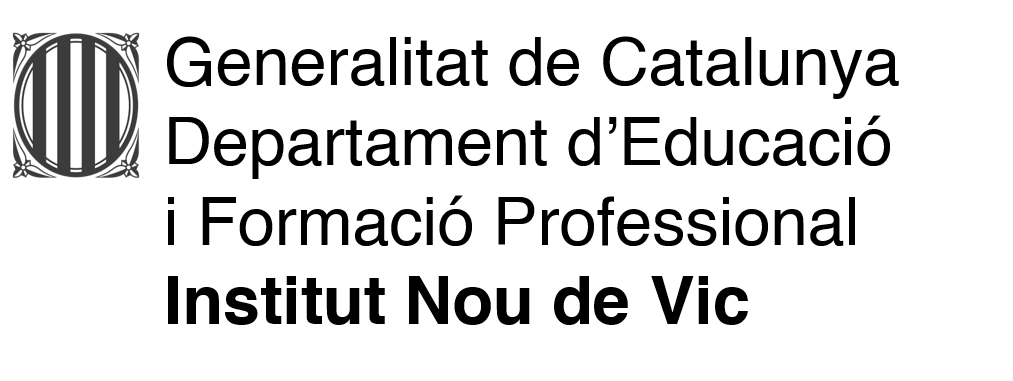
\includegraphics[height=1.8cm]{Logo_Departament.png}} 
\fancyhead[R]{
\includegraphics[height=1.8cm]{Logo_Institut.png}}
\fancyfoot[C]{Pàgina \thepage\ de \pageref{LastPage}}
\renewcommand{\headrulewidth}{0.4pt}

\begin{document}

% --- CAPÇALERA D'IDENTIFICACIÓ ---
\begingroup
\renewcommand{\arraystretch}{2.2}
\begin{tabularx}{\textwidth}{|X|p{4cm}|}
    \hline
    \textbf{Nom i cognoms:} & \textbf{Grup:} \\ \hline
    \textbf{Activitat: Funcions Fitxa 2 - Els Radians i la Circumferència} & \textbf{Data:} \\ \hline
\end{tabularx}
\endgroup

\section*{1. Conversió d'angles}
Recordant que $360^\circ = 2\pi$ rad (o $180^\circ = \pi$ rad), realitza les següents conversions:

\begin{enumerate}[label=\alph*)]
    \item Passa a \textbf{radians} (en funció de $\pi$): $30^\circ, 45^\circ, 60^\circ, 90^\circ, 120^\circ$ i $210^\circ$.
    \item Passa a \textbf{graus sexagesimals}: $\frac{\pi}{4}$ rad, $\frac{\pi}{3}$ rad i $\frac{5\pi}{6}$ rad.
\end{enumerate}

\section*{2. Taula de valors i mètode}
Fes una taula com aquesta al teu resum on es mostri l'equivalència dels angles principals de la circumferència goniomètrica en radians i anota l'equivalència per saber com es converteix d'una a l'altre.:

\begin{center}
\renewcommand{\arraystretch}{1.5}
\begin{tabular}{|l|c|c|c|c|c|c|c|c|}
\hline
\textbf{Graus ($^\circ$)} & $0^\circ$ & $30^\circ$ & $45^\circ$ & $60^\circ$ & $90^\circ$ & $180^\circ$ & $270^\circ$ & $360^\circ$ \\ \hline
\textbf{Radians (rad)} & & & & & & $\pi$ & & $2\pi$ \\ \hline
\end{tabular}
\end{center}

\section*{3. Quantes vegades hi cap el radi?}
\begin{enumerate}[label=\textbf{\alph*)}]
    \item Quantes vegades cap el radi en una circumferència de radi $r = 3$ cm?
    \begin{itemize}
        \item Calcula el seu perímetre ($L = 2\pi r$).
        \item Quants cops cap el radi ($r = 3 cm$) en aquest perímetre?.
        \item \textit{Ajuda:} Si no ho veus clar, dibuixa un segment recte amb la mida del perímetre i posa segments de 3 cm (radi) un darrere l'altre. Quants en necessites? Quina operació has de fer?
    \end{itemize}
    \item Quants cops cap el radi si la circumferència fa $5$ cm de radi?
    \item I si en fa $7$ cm?
\end{enumerate}

\textbf{Reflexió final:} Com es relaciona aquest valor constant que has trobat ($\approx 6,28$) amb $2\pi$ i la definició de radiant?

\end{document}